\documentclass[11pt,journal,compsoc]{IEEEtran}

\usepackage[T1]{fontenc}
\usepackage[utf8]{inputenc}
\usepackage[french]{babel} % Global stuff set to french
\usepackage{tcolorbox}

\begin{document}


\title{Open Wifi Localizator}
\author{Rémy Detobel, Denis Hoornaert, Nathan Liccardo, Robin Petit\\ Université libre de Bruxelles, Département des sciences informatiques, Bruxelles}

\maketitle

%\newpage

\begin{abstract}
  blablabla...
\end{abstract}
\begin{IEEEkeywords}
  Computer Society, IEEEtran, journal, \LaTeX, paper, template.
\end{IEEEkeywords}
\section{Introduction}
\section{Modélisation}
  \subsection{Graphe}
  \subsection{Recherche du plus court chemin}
    \subsubsection{A*}
    \subsubsection{Dijkstra}
\section{Localisation}
  \subsection{Introduction aux Wifi}
    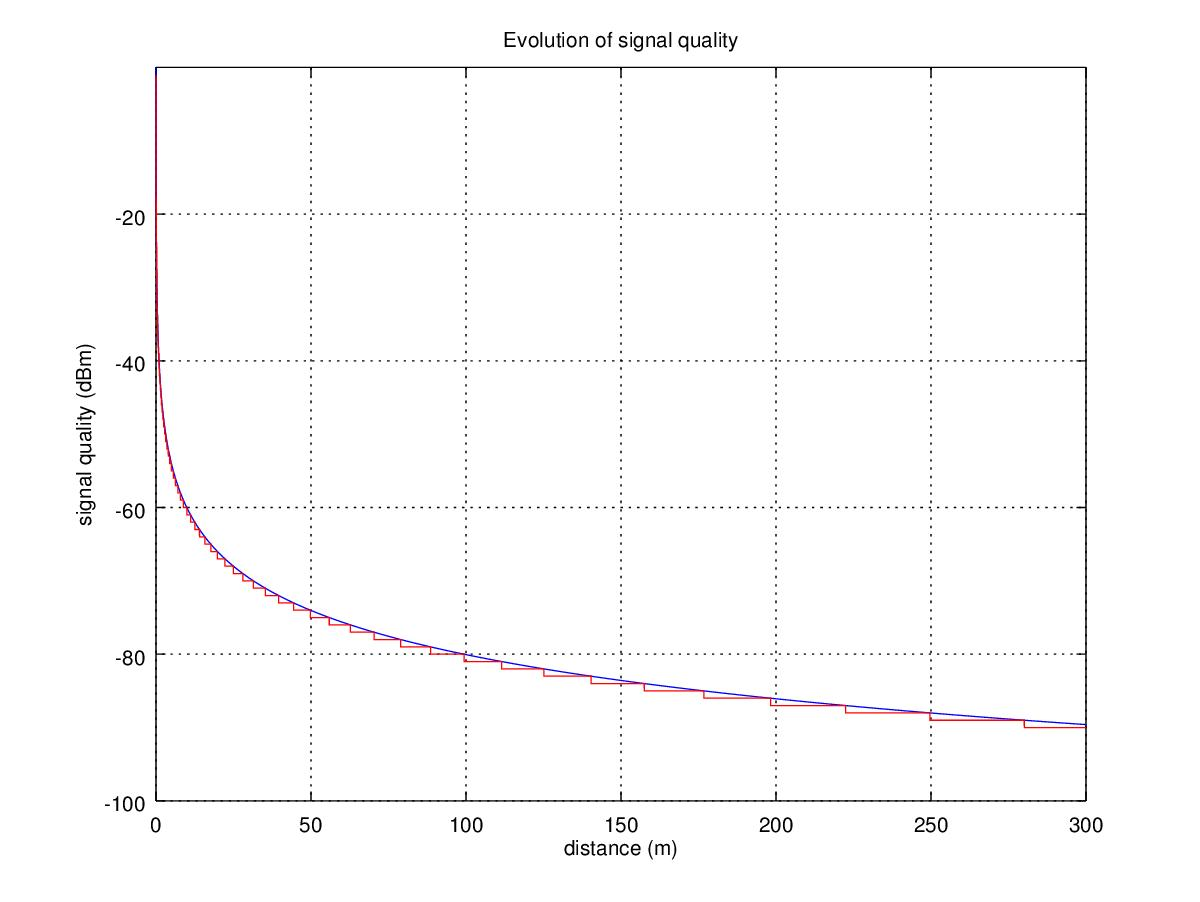
\includegraphics[scale=0.4]{images/signal-propagation.jpg}
  \subsection{Problème rencontrer par l'utilisation des Wifi}
  \subsection{Méthodes}
    \subsubsection{Trilateration}
    \subsubsection{Localisation via une Signal strength map}
      \paragraph{Méthode utilisant les processus Gaussiens}
      \paragraph{Méthode utilisant les maximum de vraisemblabilité}
        Comme mentionné plus haut, on va faire un ensemble de mesures pour chaque point du graphe et ainsi construtuire la base de données sur laquelle se basera notre méthode de localisation. Pour la méthode présente, on notera une mesure comme suit :
        \begin{equation}
          S^{(i)}=\{b_{1}, b_{2}, ..., b_{n}\} \hspace{1cm} \forall j \in [1, k]
        \end{equation}
        Où :
        \begin{itemize}
          \item $n$ est le nombre de points d'accès détectés lors de la mesure.
          \item $b_{i}$, le $i^{eme}$ point d'accès detécté, est défini comme un tuple $(a_{i}, S_{i})$ décrivant respectivement l'identifiant d'un point d'accès et la qualité de signal perçue.
        \end{itemize}
        
        On prend plusieurs mesures pour un même point car il existe des variations de qualité de signal au cour du temps. En faisant de la sorte, on se donne une idée de la qualité d'un signal à un point du graphe. On notera ces "mesures moyennes" comme suit :
        \begin{equation}
          \bar{S} = \{(a_{1}, \bar{S}_{1}), ..., (a_{n}, \bar{S}_{n})\}
        \end{equation}
        Où :
        \begin{itemize}
          \item $\bar{S}_{i} = \frac{1}{k}\sum\limits_{j = 1}^{k} S_{i}^{i} \hspace{1cm} \forall i \in [1, n]$
        \end{itemize}
        Cependant, considérer seulement la moyenne comme util statistique n'est pas suffisant due aux bruits et interférences pouvant survenir (voir section précédente). Pour pallier à ce problème, on cacule aussi la variance (noté $v$) pour chaque point du graphe. Ainsi, on obtiendra une nouvelle forme appellée ensemble charactéristique qui est définit comme suit :
        \begin{equation}
          S^{*} = \{(a_{1}, \bar{S}_{1}, v_{1}), ..., (a_{n}, \bar{S}_{n}, v_{n})\}
        \end{equation}
        Où :
        \begin{itemize}
          \item $v_{i} = \frac{1}{k-1}\sum\limits_{j = 1}^{k}(S_{i}^{(j)}-\bar{S}_{i}) \hspace{1cm} \forall i \in [1,n]$
        \end{itemize}
        On peut donc définir notre base de données (notée $\mathcal{D}$) comme l'ensemble des points du graphe (noté $L$) pour lequel il existe un ensemble charactéristique. Soit : 
        \begin{equation}
          \mathcal{D} = \{L_{1}, L_{2}, ..., L_{3}\}
        \end{equation}
        Où :
        \begin{itemize}
          \item $\dim(L_{i})$, le nombre de points d'accès à cette position, est noté $n_{i}$
          \item $S_{i}^{*}$ est l'ensemble charactéristique de $L_{i}$ 
        \end{itemize}
        
        Une fois la base de données remplie, on peut passer à l'étape dites d'exploitation. Il s'aggit du processus qui sera utilisé par une personne pour pouvoir se localiser.\\
        Le processus va déduire la position de l'utilisateur sur base de la base de données préalablement crée (notée $\mathcal{D}$) et sur base d'une mesure qu'il aura effectuée (notée $S'$). La nature de cette mesure pouvant soit être de la forme (1) ou (2).\\
        Le processus va déterminer une position $\hat{L}$ appartenant $\mathcal{D}$ pour laquelle la probabilité que l'utilisateur se trouve proche de ce point est la plus grande. Pour se faire, on va calculer, pour chaque élément appartenant à $\mathcal{D}$, un score noté $Z$ et considérer, comme solution à notre problème, le point conrespondant au score $Z$ minimal car le score $Z$ minimal représent la vraisemblabilité maximale comme prouvé dans l'article (Mettre référence). Le score $Z$ est définit comme suit :
        \begin{equation}
          Z_{i} = \sum\limits_{j = 1}^{n_{i}}\bigg(\frac{(\bar{S}_{ij}-S'_{j})^{2}}{v_{ij}}\bigg)
        \end{equation}
        Où :
        \begin{itemize}
          \item $\bar{S}_{ij}$ est la moyenne de la qualité de signal du $j^{eme}$ point d'accès
          \item $v_{ij}$ est la variance de la qualité de signal du $j^{eme}$ point d'accès
          \item $S'_{j}$ est la qualité de signal du $j^{eme}$ point d'accès de la mesure effectué par l'utilisateur
        \end{itemize}
        
        \begin{tcolorbox}[title = Mesures parasites]
          Dans cette article, on défini une mesure parasite comme la détection d'un point d'accès qui n'apparaitrait que très rarement lors de la prise de mesures. On qualifira un point d'accès comme tel si le nombre de fois qu'il a été détecté est inférieur à un seuil fixé.
          \\
          Ce cas de figure survient pour des points d'accès situés à une distance telle qu'ils ne sont pas toujours percus mais qui, dans le cas contraire, présentent des qualités de signal in férieur à $-90 dBm$.
        \end{tcolorbox}
      \paragraph{Monte carlo}
      \paragraph{Amélioration par l'utilisation de filtres}
      \paragraph{Amélioration par l'estimation de qualité de signal}
\section{Discussion et limitations}
\section{Conclusion}

\begin{thebibliography}{9}
  \bibitem{ssm}
    Matteo Cypriani, Frédéric Lassabe, Philippe Canalda, François Spies,
    \emph{Wi-Fi-Based Indoor Positioning: Basic Techniques, Hybrid Algorithms and Open Software Platform}.
    2010.
  \bibitem{Roumanie}
    Bianca BOBESCU, Marian ALEXANDRU
    \emph{Mobile indoor positioning using Wi-fi localisation}.
    Transilvania University, Brasov, Romania,
    2015.
  \bibitem{trilateration}
    OnkarPathak, Pratik Palaskar, Rajesh Palkar, Mayur Tawari,
    \emph{Wi-Fi Indoor Positioning System based on RSSI Measurements from Wi-Fi Access Points A Trilateration Approach}.
    International Journal of Scientific \& Engineering Research,
    2014.
  \bibitem{GaussianProcessesFerris}
    Brian Ferris, Dirk Hähnel, Dieter Fox,
    \emph{Gaussian Processes for Signal Strength-Based Location Estimation}.
    University of Washington, Department of Computer Science \& Engineering, Seattle, WA Intel Research Seattle, Seattle, WA.
\end{thebibliography}

%---------- SCANNING ----------
%# www.mdpi.com/1424-8220/15/9/21824/pdf
%https://www.researchgate.net/publication/224198838_Wi-Fi-based_indoor_positioning_Basic_techniques_hybrid_algorithms_and_open_software_platform
%x https://fruct.org/publications/abstract16/files/Shc1.pdf
%http://www.afahc.ro/ro/revista/2015_1/119.pdf
%x http://file.scirp.org/pdf/CN_2013071010352139.pdf
%http://www.ijser.org/researchpaper%5CWi-Fi-Indoor-Positioning-System-Based-on-RSSI-Measurements.pdf
%https://www.researchgate.net/profile/Suhailan_Safei/publication/230771403_INDOOR_POSITION_DETECTION_USING_WIFI_AND_TRILATERATION_TECHNIQUE/links/5513e9120cf2eda0df3031f0.pdf
%http://www.ee.ucl.ac.uk/lcs/previous/LCS2005/12.pdf
%http://www.int-arch-photogramm-remote-sens-spatial-inf-sci.net/XXXVIII-4-C26/1/2012/isprsarchives-XXXVIII-4-C26-1-2012.pdf
%---------- LOCALISATION ----------
%http://www.roboticsproceedings.org/rss02/p39.pdf
%https://venturi.fbk.eu/wp-content/uploads/2011/10/AraMes_WIMOB_2014.pdf
%http://www.tik.ee.ethz.ch/file/2490a7adb6a163b9c5be1510d033870a/sawn05.pdf
%https://felixduvallet.github.io/pubs/2008-WiFi-IROS.pdf
%http://www.cs.cmu.edu/~mmv/papers/10icra-joydeep.pdf
%https://papers.nips.cc/paper/2541-gpps-a-gaussian-process-positioning-system-for-cellular-networks.pdf
%http://www-cs.stanford.edu/people/dstavens/icra11/huang_etal_icra11.pdf
%https://www.ncbi.nlm.nih.gov/pmc/articles/PMC5017359/
%http://www.robot.t.u-tokyo.ac.jp/~yamashita/paper/E/E293Final.pdf

\section*{Annexes}

\end{document}
